\begin{multicols}{2}
	
	\begin{center}
		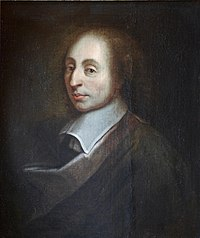
\includegraphics[height=.9\linewidth]{./IMG/Blaise_Pascal_Versailles.JPG}
	\end{center}


\vfill
\columnbreak

Em 1642 o matemático francês Blaise Pascal, que era filho de um cobrador de impostos, inventou uma máquina automática de cálculos para agilizar o trabalho do seu pai.

	\begin{center}
	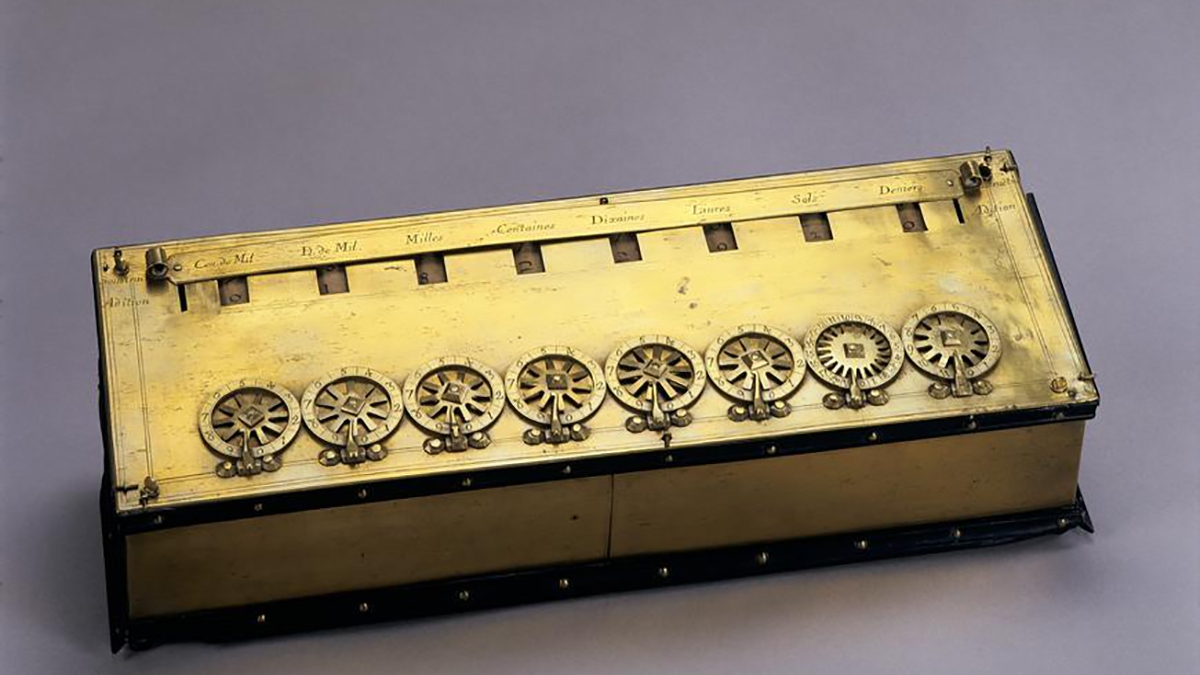
\includegraphics[width=\linewidth]{./IMG/pascaline.jpg}
\end{center}

\end{multicols}

\vfill
\pagebreak
